\chapter{Penetrator}

* What kind of ice can we expect? Mud, silt etc?

\section{Drilling Methods}

\autsubsection{Mechanical Drilling}{Morten Lykke Hilligsøe}
On earth, drilling is by far the most common way of penetrating ice and has proved a viable way for recovering ice core samples at depths of up to 3.768km, reaching the underground lake Vostock, much like the mission at hand. Drilling has previously reached depths of 12.262km, and because of e.g. the oil drilling industry, experience and components are readily available. It is therefore obvious to look at the possibility of drilling through the ice on Europa.

To compare with other ice penetration methods, the following key parameters are evaluated:
\begin{itemize}
    \item Energy
	\item Time
	\item Weight
\end{itemize}
The energy required for a drill solution consists of two parts: the cutting energy and the potential energy required to move the ice. To calculate these energies, the following assumptions have been made:
\begin{itemize}
	\item Probe length:   $2m$
	\item Probe diameter:   $30cm$
	\item Europa surface gravity:   $1,3m/s^2$
	\item Europa ice density:   $124kg/m^3$
	\item Specific ice cutting energy:   $16MJ/m^3$
\end{itemize}
For cutting energy, the key parameter is the specific cutting energy. This parameter is assumed to be $16MJ/m^3$, as measured by \footnote{Greenland Ice Core: Geophysics, Geochemistry, and the Environment, Volume 33,  Chester C. Langway, Hans Oeschger, W. Dansgaard}. Other sources, e.g. \footnote{Life in Extreme Environments, Ricardo Amils, J. Cynan Ellis-Evans, Helmut Hinghofer-Szalkay}, have measured specific cutting energies of similar size, at $20MJ/m^3$.

The result is a cutting energy of:
\begin{equation}
    E_{Cut} = A \cdot E_{Specific}
\end{equation}
\begin{equation}
    E_{Cut} = (0.15m)^2 \cdot \pi \cdot 16MJ/m^3 \cdot 1000m/km = 1.130 MJ/km
\end{equation}
The potential energy required to move the ice, will have to at least match the volume of ice which the penetrator probe displaces.  The result is a minimum potential energy of:
\begin{multline}
E_{pot} = m \cdot g \cdot h = \rho \cdot V \cdot g \cdot h\\
 = (0.15m)^2 \cdot \pi \cdot 124kg/m^3 \cdot 1.3m/s^2 \cdot 2m \cdot 1000m/km = 22.8 kJ/km
\end{multline}
Where the surface gravity of Europa is provided by \footnote{\url{https://en.wikipedia.org/wiki/Europa_(moon)}}, and the ice density $\rho$ is calculated from the value on earth at -180°C as stated in \footnote{\url{https://en.wikipedia.org/wiki/Properties_of_water}}:
\begin{equation}
\rho_{Europa} = \rho_{Earth} \cdot \frac{g_{Europa}}{g_{Earth}}
\end{equation}
\begin{equation}
\rho_{Europa} = 934kg/m^3 \cdot \frac{9.82m/s^2}{1.3m/s^2} = 124kg/m^3
\end{equation}
Compared to the cutting energy, the potential energy seems insignificant. However, this might not be a realistic assumption, since the shaved ice will most likely take up more space than the equivalent amount of solid ice, and will therefore have to either be moved additionally, or compressed. Also, the drilling equipment will most likely take up a much greater volume than the probe itself, and this energy must therefore be expected to increase in multifold.

But even if the energy required to drill through the ice is reasonable, drilling time and system weight are key parameters. Table \ref{tab:ice_core_drilling}\footnote{A Fast Mechanical-Access Drill for Polar Glaciology, Paleoclimatology, Geology, Tectonics, and Biology, Gary D. Clow and Bruce Koci}  presents these key parameter for two currently employed methods of ice drilling: Ice Core Drilling (ICD) and Hot-Water Drilling (HWD), as well as a solution based on Coiled Tubing Drillling for Ice (CTDI), which have yet to be employed in ice drilling projects. As seen from this table, drilling a 3.5km borehole can take as little as 6-8 days by using a CTDI system. However, the weights of such systems are in the tens-hundreds of tonnes, making ice drilling systems impossible to bring as payload on a rocket.

\begin{figure}[htb]
  \centering
  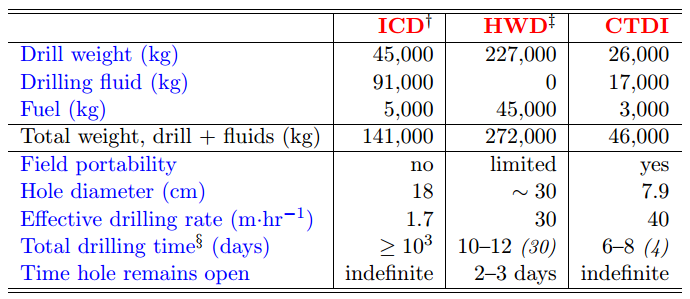
\includegraphics[width=0.7\textwidth]{figures/mlh/table_ice_core_drilling}
  \caption{Comparison of the weights and times required to drill a 3.5-km borehole through ice using ice-coring, hot-water, and CTDI drilling systems.}
  \label{tab:ice_core_drilling}
\end{figure}

Figures \ref{fig:ICD}, \ref{fig:HWD} and \ref{fig:CTDI} illustrates the three methods presented in table \ref{tab:ice_core_drilling}.

\begin{figure}[htb]
  \centering
  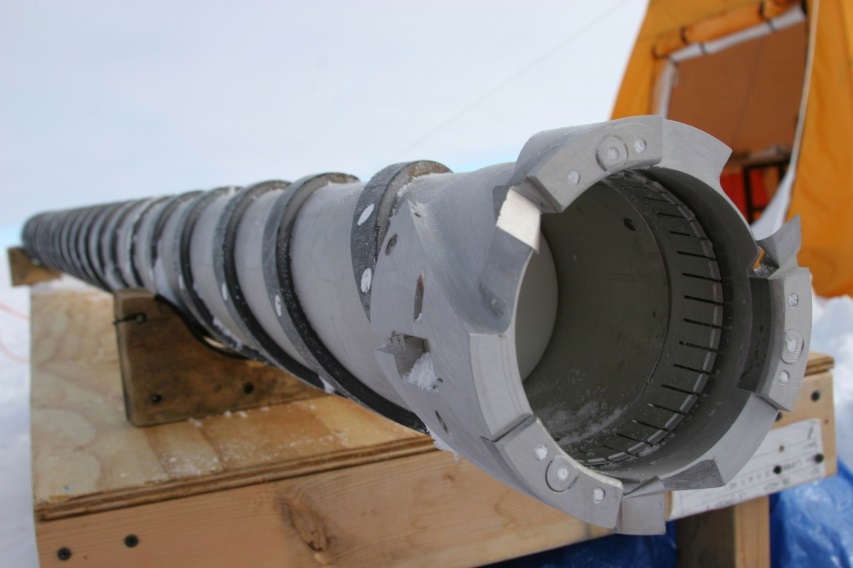
\includegraphics[width=0.5\textwidth]{figures/mlh/ICD}
  \caption{The hollow drill of an Ice Core Drilling, which enables researchers to retrieve pure ice core samples.}
  \label{fig:ICD}
\end{figure}
\begin{figure}[htb]
  \centering
  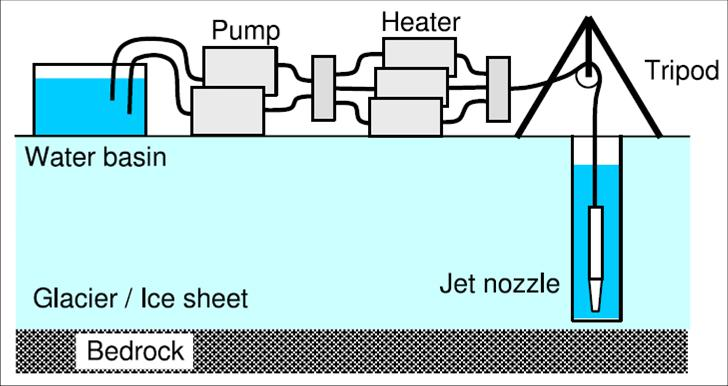
\includegraphics[width=0.5\textwidth]{figures/mlh/HWD}
  \caption{Principles of Hot Water Drilling in ice.}
  \label{fig:HWD}
\end{figure}
\begin{figure}[htb]
  \centering
  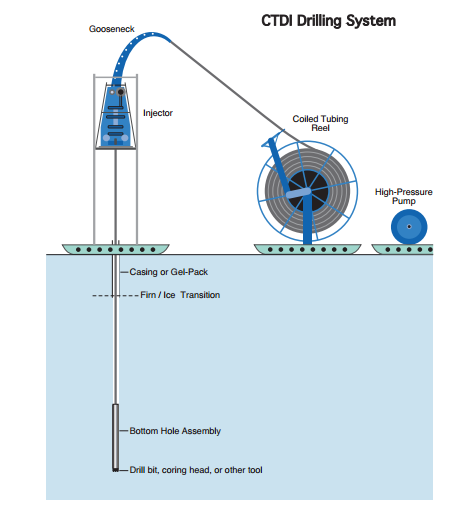
\includegraphics[width=0.6\textwidth]{figures/mlh/CTDI}
  \caption{Principles of Coiled Tube Drilling in Ice.}
  \label{fig:CTDI}
\end{figure}

\subsection{Chemical Drilling}

\subsection{Explosive Drilling}

\subsection{Sputtering}

\autsubsection{Laser Drilling}{Bhaaeddin Alhomsi and Paul Connetable}

Lasers may provide another methodto dig through the layer of ice. High-power lasers exceeding 10 kW have been developed and widely used for industry (Gapontsev et al., 2009; Richardson et al., 2010; Fujita et al., 2010). For example, a recent laboratory test using a 1.6-kW pulsed Nd:YAG 1.064 $\mu$m wavelength laser beam determined the energy required to spall, melt, and
vaporize several rock samples for oil and gas well drilling. The required energy (specific energy) depends on the absorption properties of each rock sample as well as the reflective properties of the rock surface  (Gahan and Parker, 2001; Xu et al., 2003). A new laser-mechanical bit for laser spallation of rock to give an optimum drilling mechanism
was found to reduce rig time and increase drilling efficiency (Pooniwala, 2006).More recently, a 20-kWlaserwas delivered through a 1500 m-long optical fiber cable and shown to be able to efficiently drill oil and gas wells (Hecht, 2012). Finally, in the project VALKYRIE,
ice was drilled by a self-contained "intelligent ice penetrator", a 5 kW laser at 1070 nm wavelength (Siegel et al., 2013)(Stone et al., 2014).
Test of VALKYRIE between 2010 and 2013 used high-power optical energy transfer over km-scale distances and tested the feasibility of a vehicle deployed optical waveguide. Thus, a laser-drill system may be useful for ice-sheet applications, including the search for life in extreme environmental conditions here on Earth as well as outer planets.
With continual improvements, laser drilling may develop advantages over other methods for ice.We investigate here the behaviour of laser melting of ice and snow with an infrared laser for the potential use as a drill.

\subsubsection{Characteristics of light absorbance in ice}

The first step before selecting a laser is to analyze the spectral absorption of the medium we want to dig through. Therefore, the ice transmittance spectrum is displayed in Figure \ref{IceAbsorbance}. One can observe on this figure peaks of absorption, at around $10^{-5}~m$, and around $6\times10^{-5}~m$. The best suited lasers for digging through ice would have to emit at these frequencies.

Hence, we use a $CO_2$ laser, which is a relatively inexpensive common infrared gas laser (Patel, 1964) with fundamental lines from 9.2 to 10.8 $\mu$m and used in both pulse and continuous wave (CW) mode. For ice, an earlier study demonstrated the potential of $CO_2$ laser irradiation to help breakup nautical sea-ice (Clark et al.,  1973), but the laser has apparently not previously been used for snow and ice drilling.

\begin{figure}[htb]
\centering
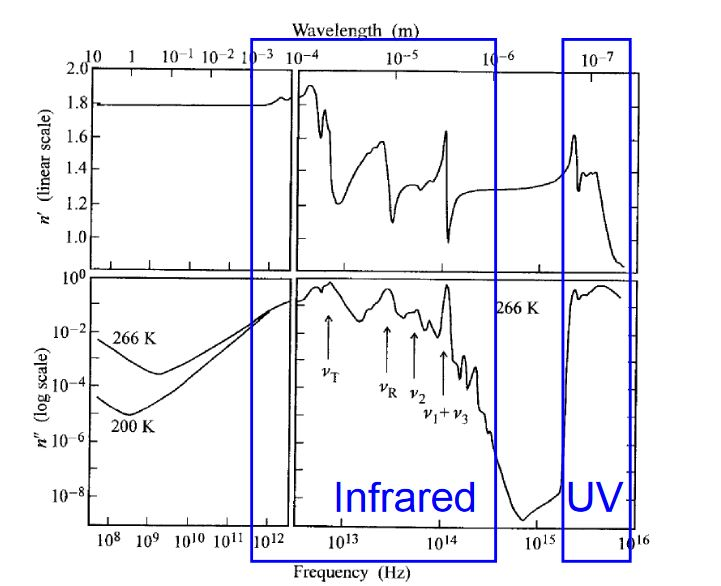
\includegraphics[width=.48\textwidth]{figures/laser-drilling/iceabsorbance}
\caption{Reported values of transmittance in ice}
\label{IceAbsorbance}
\end{figure}

The absorption of light in ice depends on the complex refractive index of ice. According to data in a previous study (Warren and Brandt, 2008), the absorption coefficient of ice significantly increases from the near- to mid-infra-red region, reaching a value of about $\unit[628.3]{cm^{-1}}$ at the $CO_2$ laser wavelength of 10.6 $\mu$m. Ice absorbs almost 100\% of the light intensity at 10.6 and 1.064 $\mu$m within a penetration distance of 0.01 and 2 cm, as shown in Figure \ref{fig:bh1}.

\begin{figure}[htb]
\centering
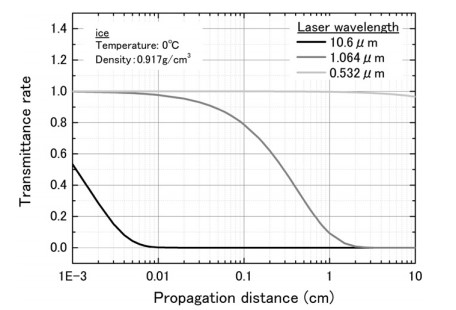
\includegraphics[width=.48\textwidth]{figures/laser-drilling/bh1.jpg}
\caption{Characteristics of light absorbance in ice}
\label{fig:bh1}
\end{figure}

\subsubsection{Melting studies of ice and snow by $CO_2$ laser}

A $CO_2$ laser can be used to melt ice. The $CO_2$ laser at 10.6 $\mu$m (25.5 W) and a beam diameter of 1.0 cm, a wavelength at which ice strongly absorbs, to drill (via melting) through ice. The resulting drilling speed is measured at several irradiation intensities, ice-snow densities, and beam angles relative to the horizontal axis.
The melting speed increases with increasing laser intensity and with decreasing ice density, as shown in Figure \ref{fig:bh2}. The melting speed ratio between ice ($\unitfrac[917]{kg}{m^3}$) and the lowest-density snow ($\unitfrac[153]{kg}{m^3}$) is 4-5, slightly less than the value of \~6 expected from the density ratio \cite{lasermelt}. The reason for this discrepancy could be explained by the snow having a greater reflectivity than solid ice. The melting speed decreases with increasing snow density.

\begin{figure}[htb]
\centering
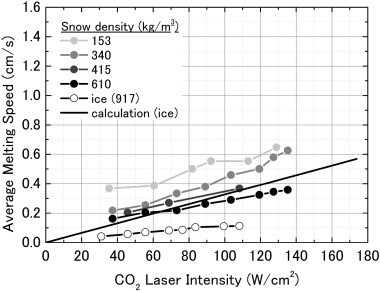
\includegraphics[width=.48\textwidth]{figures/laser-drilling/bh2.jpg}
\caption{Relation between laser intensity and melting speed}
\label{fig:bh2}
\end{figure}

\subsubsection{Results}

Unfortunately, the experimental results indicate that the melt-water accumulates in the hole and reduces the melting speed of ice and a pump system could not be installed due to a high distance.
Moreover, since the energy source brought in the penetrator is a RTG, using a laser would require to transform the thermal energy produced by the RTG in electric energy. Such a conversion has an efficiency of about 20~\%. If we add to that the fact that the best $CO_{2}$ lasers also have efficiencies up to only 20~\%, the best efficiency achievable on this drilling method is of about 4~\%with the current technology. This is still while assuming that the ice absorbs all of the energy sent by the laser, which is not the case. It means that the efficiency of such a drilling method would be extremely low, and thus not indicated for our mission.
In future studies, it will be necessary to investigate quantitatively several additional factors. These include the optical-fiber coupled laser intensities required for deep drilling, and a method to pump melted water. Despite these hurdles, laser drilling is a promising technology for ice drilling. Lasers are indeed capable of delivering very high powers precisely. Furthermore, the main reason for low $CO_{2}$ lasers' efficiency is the power consumed for cooling the body of the laser. This efficiency could then go up if a laser specifically designed for our mission was done, since it could use the cold surroundings of the penetrator to cool down.


\subsection{Light Concentration Drilling}

\subsection{Melting}

* Water transportation from tip to the end of the penetrator (ref section about convection flow)

* Should measure flow of the water - descent rate

* Water flow to the instruments. Will have to use a pump in order to increase the flow rate.

* Measure conductivity of the water.

\section{Selected Design}

* Sketch of overall design (use 3D models for the ice melting simulations)

\subsection{Melting through the ice} % Lukas, KSL

\subsection{RTG on Top}

\subsection{RTG on Bottom}

* How do we protect the rest of the instruments against the radiation?

\subsection{RTG design}

* Can we make it smaller?

* Thermal design

\subsection{Thermal Design}

\subsection{Water Convection}

\subsection{Anchor Design}

\subsection{Anchoring and Deployment}

* Ref to composition of the ice and theory about lakes?

\subsection{Submarine}

\section{Mechanisms and Instrumentation}

\subsection{Navigation and Dirigibility}

\subsection{Detection of Depth and End of Ice Column}

* Echo sounder etc

\section{Communication Systems}

\subsection{Ice Losses}
As we expect, Europa's subsurface consists mainly of several kilometers of ice, which we want to penetrate with electromagnetic waves to establish the communication link between the penetrator and the lander vehicle. Fortunately, a lot of research has been made in the recent decades on how efficient an electromagnetic wave can penetrate different ice layers and on which parameters can affect this propagation. These principles are applied widely in subsurface radar sounding that take place in polar areas, but also in planetary exploration (Mars). For a wide range of frequencies, ranging from MHz to GHz, dielectric losses of ice are independent of frequency. By that it is meant that, the number of wavelengths, which can penetrate into ice before being attenuated to a given fraction of its initial amplitude ($1/e$ of initial amplitude) is approximately the same regardless of frequency. The above implies that the longer the wavelength, the deeper the radar signal can penetrate before being attenuated below the detection of our equipment. Thus, deep ice penetration requires that the radar operates at the lowest possible frequency. 

\paragraph{Dielectric properties of ice}
(For the following two paragraphs \cite{Kofman_2010} has used as main reference.)The permittivity $\epsilon$ of a material is a property describing how much more energy is stored though change separation than in vacuum. Frequency dependence of permittivity occurs because change separation does not happen instantaneously. Changes separate with finite velocities, thus if the external field is reversing polarity too quickly the changes cannot move fast enough to keep up. The frequency at which the charges fully separate and are in constant motion is called the relaxation frequency. At frequencies below the relaxation frequency the permittivity plateaus at the low frequency limit (static) $\epsilon_{s}$, which is often call dielectric constant. At high frequencies above the relaxation frequency the permittivity plateaus at the high frequency limit $\epsilon_{\infty}$. Moreover, ice crystal formation has an impact on polarization, which primarily depends on temperature.

Debye model takes into account the above mentioned theory about dielectric constant of ice and is described by the following equations: 

\begin{equation}
    \epsilon=\epsilon_{\infty}+\Delta \epsilon \frac{\Delta \epsilon}{1+j \omega \tau}
    \label{dielectric}
\end{equation}

, where $\omega = 2\pi f$, $\Delta \epsilon=\epsilon_{s} -\epsilon_{\infty}$ and $\tau$ is the dielectric relaxation time. \\
The permittivity is a complex function of frequency and usually is described by its real and imaginary part.

\begin{equation}
    Re (\epsilon)=\epsilon_{\infty}+\Delta \epsilon \frac{\Delta \epsilon}{1+ \omega^2 \tau^2}
    \label{real}
\end{equation}

\begin{equation}
    Im (\epsilon)=\frac{\Delta \epsilon\ \omega\  \tau}{1+ \omega^2 \tau^2}
    \label{imag}
\end{equation}
The loss tangent (tan $\delta$) is defined by the ratio of these two parts and characterizes the attenuation of the electromagnetic waves in a medium due to ohmic conductivity $\sigma$. 

\begin{equation}
    tan \delta=\frac{Re(\epsilon)}{Im(\epsilon)}=\frac{\sigma}{\omega\ Re(\epsilon)}
    \label{tan}
\end{equation}
The conductivity $\sigma$ of the medium is directly proportional to the imaginary part of the dielectric constant.

Because of the complexity of equations (\ref{dielectric} - \ref{tan}) an approximated expression has been developed to compute the attenuation.

\begin{multline}
    a=0.129 \sqrt{Re(\epsilon)}\ f (\sqrt{1+tan^2 \delta}-1)^{1/2} \approx \\
    \approx 0.091 \sqrt{Re(\epsilon)}\ f\ tan \delta \approx 0.0009\ \sigma\ dB/m
    \label{losses}
\end{multline}
where, $\sigma$ is in $\mu S m^{-1}$. As one can see from eq. (\ref{losses}), attenuation's value is directly proportional to frequency, or in other words to the conductivity of the medium. Additionally, the static dielectric constant of pure ice is heavily depended on the orientation of electric field with respect to the crystal's axis. The effect of pressure is about 1\% per kbar for polycrystalline ice \cite{Kofman_2010}. The above formulas and their approximations concerning the electromagnetic waves can be used adequately for very low temperatures, as the ranges we are interested.

Nevertheless, the losses due to pure ice are well documented in bibliography, there is a big gap regarding ice impurities on icy moons. The absence of these data are due to uncertainties and lack of knowledge of the physical nature of impurities on these satellites. This problem was studied by  Moore \cite{Moore_2000} and Chyba \cite{Chyba_1998} for Europa. Moore considered three types of water ice on Europa, produced by three basic processes occurring on Earth. The first one is meteoric ice formed by atmospheric precipitations, sea ice formed by the freezing of water close to the atmospheric interface and marine ice forming beneath ice shelves directly from ocean water. Moore concluded that similar processes are likely to occur on Europa as well, and that the most probable form of ice would be marine ice. In figure \ref{impurities} Moore sums up the attenuation from different type of impurities in ice \cite{Moore_2000}.

\begin{figure}[ht]
\centering
\label{impurities}
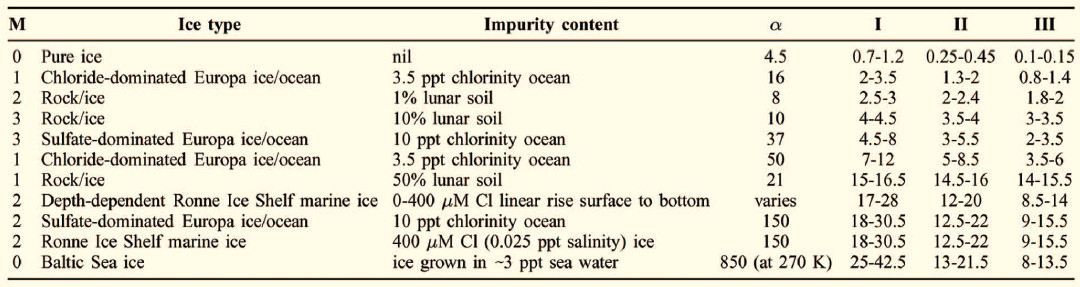
\includegraphics[width=1\textwidth]{figures/Moore2.jpg}
\caption{Attenuation, $a$, is in dB/km at 251 K and corresponds to the one way attenuation due to  ice impurities, in case of a sounding radar. Columns I, II, and III are computed one-way attenuation, in dB/km, for ice shells with base temperatures of 270, 260, and 250 K, respectively. The range of values for each of these corresponds to surface temperatures of 50 and 100 K. These values are independent of shell thickness since the temperature profile is stretched to the ice thickness. The M column represents the plausibility of the ice type for Europa; 0 is least likely while 3 is more likely, given the present understanding
of Europa. The distribution coefficients $k_{0}$ and $k_{MI}$ affecting the marine ice models come from laboratory experiments \cite{Moore_2000}. \textbf{+ appendix}}
\end{figure}
The above calculations data are not taking into account a possible scattering mechanism of electromagnetic wave due to ice layers that can exist in the crust. The scattering effect has a significant impact on the attenuation level and depends strongly on the dimensions of cavities in the medium compared to the wavelength. The two main mechanisms of scattering coming from the ice crust are surface scattering and scattering by volume irregularities. Both these effects can change considerably the penetration depth of the wave into the ice, but also the ratio of any subsurface echo to surface clutter. As we can understand the scattering depends strongly on the wavelength and surface parameters of the body under investigation. 

The conclusion is that the expected one way attenuation because of impurities of ice is in the range 1-8 dB/Km and this number is independent of the frequency. Although, the frequency dependence of attenuation due to scattering mechanisms dictates the use of as low frequencies as possible in order to achieve a deep penetration. The main bottlenecks in that case are two. The first one is that the choice of frequency has an influence on the characteristics of instrumentation and especially on the size of the antenna and the second one is Jupiter's radio emissions spectrum. Figure \ref{J_spec} depicts how Jupiter's activity affect the electromagnetic environment of its moons. Clearly can be seen that frequencies from almost zero Hz up to 50 MHz are dominated from Jupiter's radio emissions. Thus, the exact choice of frequency results in a trade off between science requirements and technical limitations taking into account also the physical constraints of the environment under research. 

\begin{figure}[ht]
\centering
\label{J_spec}
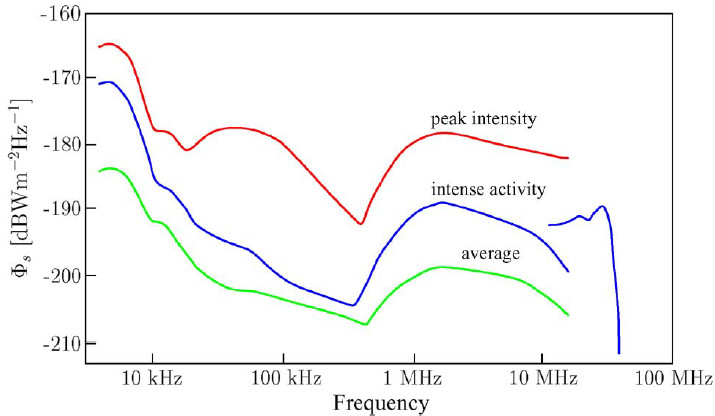
\includegraphics[width=0.7\textwidth]{figures/below100.jpg}
\caption{Jupiter radio spectrum based on Cassini-RPWS data,
normalized to a distance of 1 AU. Green curve: rotation averaged
emission. Blue curve: rotation averaged emission at times of intense
activity. Red curve: peak intensities during active periods. \cite{Grie_meier_2005}}
\end{figure}


\begin{figure}[ht]
\begin{center}
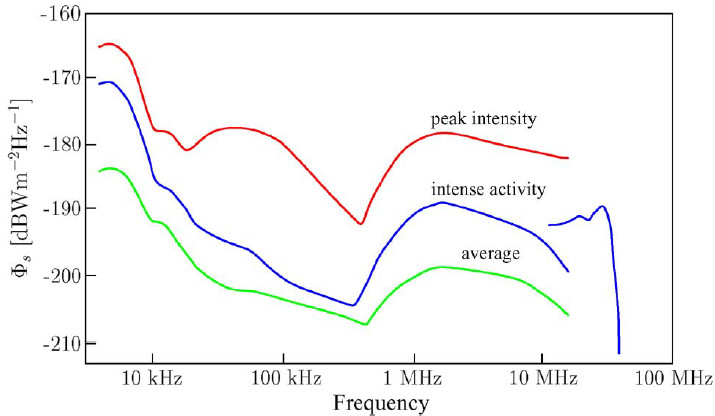
\includegraphics[width=0.7\columnwidth]{figures/below100}
\caption{Replace this text with your caption%
}
\end{center}
\end{figure}

\subsection{Communication to Lander}

\subsection{High Directivity Link}

\subsection{Relay Systems}
